\documentclass{article}
\usepackage[T1]{fontenc}
\usepackage[utf8]{inputenc}
\usepackage[portuges]{babel}
\usepackage{graphicx}
\begin{document}
	\centerline{Instituto Politécnico Cávado do Ave \linebreak}
	\vspace*{1 em}
	\centerline{Curso engenharia de Sistemas Informáticos \linebreak}
	\vspace*{1 em}
	\centerline{Sistemas Operativos e Sistemas Distribuídos\linebreak}
	\vspace*{5 em}
	
	\centerline{Autores}
	
	\vspace*{3 em}
	\centerline{Carlos Santos Nº 19432\linebreak}
	\vspace*{1 em}
	\centerline{João Rodrigues Nº 19431\linebreak}
	\vspace*{1 em}
	\centerline{João Ricardo Nº 18845 \linebreak}
	\vspace*{3 em}
	
	\centerline{\textbf{Trabalho Prático}}
	
	\vspace*{10 em}
	\centerline{Data: 29/12/2020}
	
	\newpage
	%% ----------- Pagina 2
	\centerline{\textbf{ÍNDICE}}
	\vspace*{3 em}
	
	\begin{enumerate}
		\item Parte 1 \hspace{30 em} 3 \\
		\item Parte 2 \hspace{30 em} 5\\
		\item Parte 3 \hspace{30 em} 6\\
		\item Conclusão \hspace{28,5 em} 14 \\
		\item Execução das Tarefas \hspace{24 em} 15 \\
	\end{enumerate}
	%% ----------- Pagina 3
	
	\newpage
	\centerline{\textbf{Parte 1}}
	\vspace*{1 em}
	\centerline{Implementação de um conjunto de comandos para manipulação de ficheiros}
	\vspace*{3 em}
	
	Era pretendido que se implementa-se os seguintes comandos:
	\begin{enumerate}
		\item \textbf{mostra} ficheiro - Este comando deve mostrar no ecrã o conteúdo do ficheiro indicado. 
		\item \textbf{conta} ficheiro - Este comando deve contar o número de caracteres existentes de um ficheiro.
		\item \textbf{apaga} ficheiro - Este comando deve apagar o ficheiro com o nome indicado.
		\item \textbf{informa} ficheiro - Este comando apresenta a informação do sistema de ficheiros em relação ao ficheiro dado.
		\item \textbf{acrescenta} origem destino - Este comando deve acrescentar o conteúdo da "origem" no final do "destino".
		\item \textbf{lista} [caminho] - Este comando deve apresentar uma lista de todas as pastas e ficheiros existentes no caminho indicado ou na diretoria atual se não especificado.
	\end{enumerate}
	%% pagina 4
	\newpage
	\vspace*{2 em}
	Através de chamada de funções ao sistema(\textit{system calls}). Estes comandos implementados em C serão invocados através de um interpretador de comandos.
	
	\vspace*{4 em}
	\begin{figure}[!htb]
		\centering
		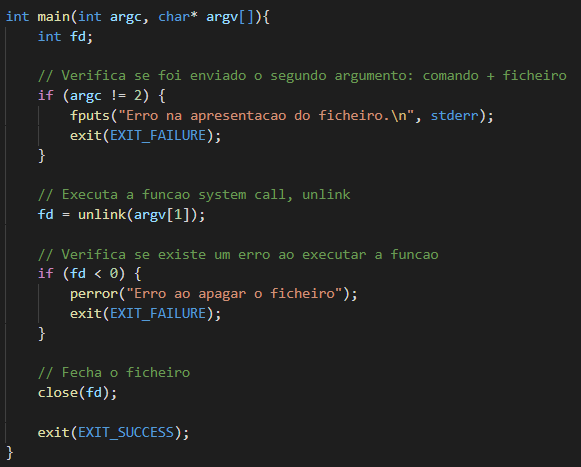
\includegraphics[scale=0.8]{apaga_parte1}
		\caption{Função Apaga}
		%%\label{Label de referência para a imagem}
	\end{figure}
	
	\footnote[1]{https://linux.die.net/man/}
	
	\newpage
	
	% ------- Pagina 5 ------
	
	\centerline{\textbf{Parte 2}}
	\vspace*{1 em}
	\centerline{Implementação de um interpretador de comandos}
	\vspace{3 em}
	
	No sentido de substituir o interpretador de comandos habitual, por um novo interpretador personalizado, era importante implementar um programa que execute o comando através de primitivas de execução genérica de processos. \\
	Cada comando deverá dar origem a um novo processo e adicionalmente, poder considerar que a execução do interpretador deve ser suspensa até ao comando indicado estar concluído. O interpretador deverá indicar sempre se o comando conclui com ou sem sucesso, através do seu código de terminação/erro. O programa deverá permitir executar vários comandos sequencialmente, isto é, um a seguir ao outro, até	o utilizador indicar o comando especial “termina” que termina esta aplicação.
	
	\vspace*{4 em}
	\begin{figure}[!htb]
		\centering
		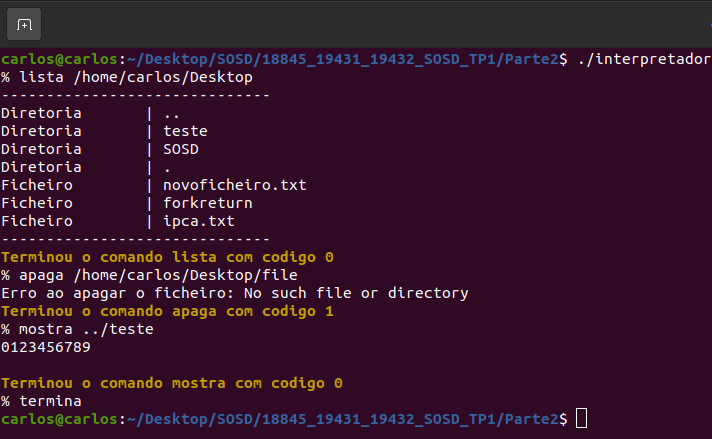
\includegraphics[scale=0.7]{interpretador_parte2}
		\caption{Funcionamento do interpretador}
		%%\label{Label de referência para a imagem}
	\end{figure}
	\newpage
	
	% ------- Pagina 6 -------
	\centerline{\textbf{Parte 3}}
	\vspace{1 em}
	\centerline{Análise de cópia de ficheiros entre máquinas virtuais}
	\vspace{3 em}
	
	
	a) Configure a sua máquina virtual, de modo a que consiga comunicar com o host
	físico (máquina real).
	\vspace{2 em}
	\begin{figure}[!htb]
		\centering
		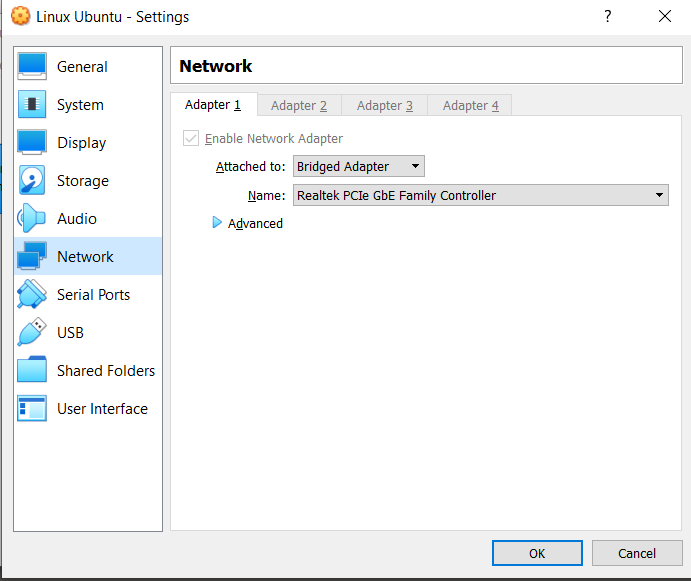
\includegraphics[scale=0.7]{tp_sosd_a1}
	\end{figure}
	
	\newpage 
	\begin{figure}[!htb]
		\centering
		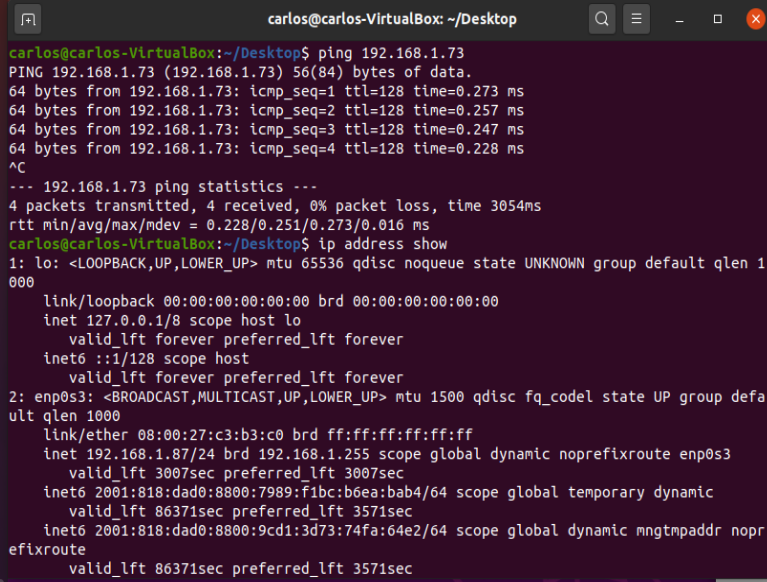
\includegraphics[scale=0.6]{tp_sosd_a2.1}
	\end{figure}

	\vspace{2 em}

	\begin{figure}[!htb]
		\centering
		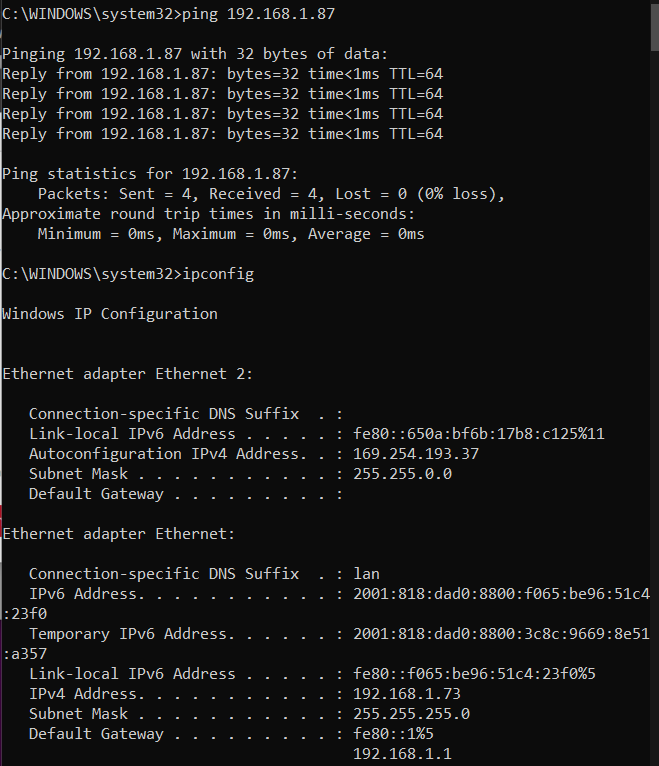
\includegraphics[scale=0.6]{tp_sosd_a2.2}
	\end{figure}
	
	\newpage
	b)Recorrendo ao comando iperf3 mostre as diferenças de transferências entre a
	máquina real e virtual, usando tcp e udp.
	\vspace{2 em}
	
	\begin{figure}[!htb]
		\centering
		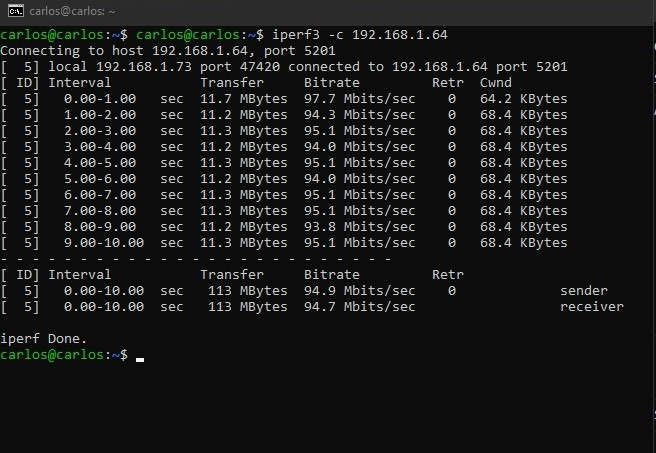
\includegraphics[scale=0.6]{tp_sosd_b1.1}
	\end{figure}
	\vspace{2 em}
	\begin{figure}[!htb]
		\centering
		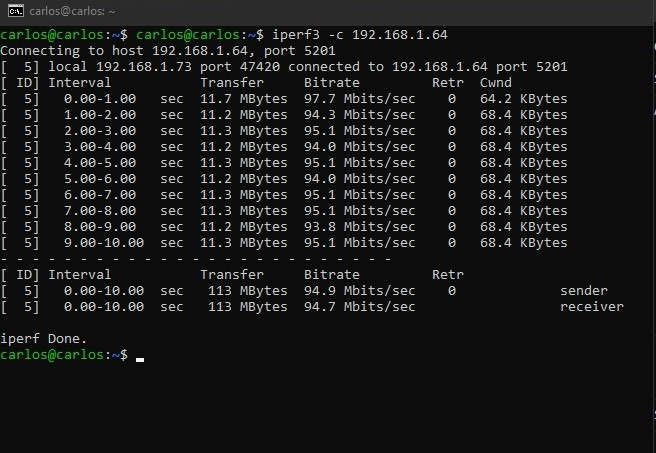
\includegraphics[scale=0.6]{tp_sosd_b1.1}
	\end{figure}
	
	\newpage
	c) Instale um servidor web (nginx ou apache) e mostre os resultados de um teste
	de carga ao “url /”, simulando 10 clientes em simultâneo e 500 pedidos cada
	um, utilizando o utilitário ab ou jmeter, sendo que o jmeter terá um acréscimo
	de 0.3 valores.
	\vspace{2 em}
	
	\begin{figure}[!htb]
		\centering
		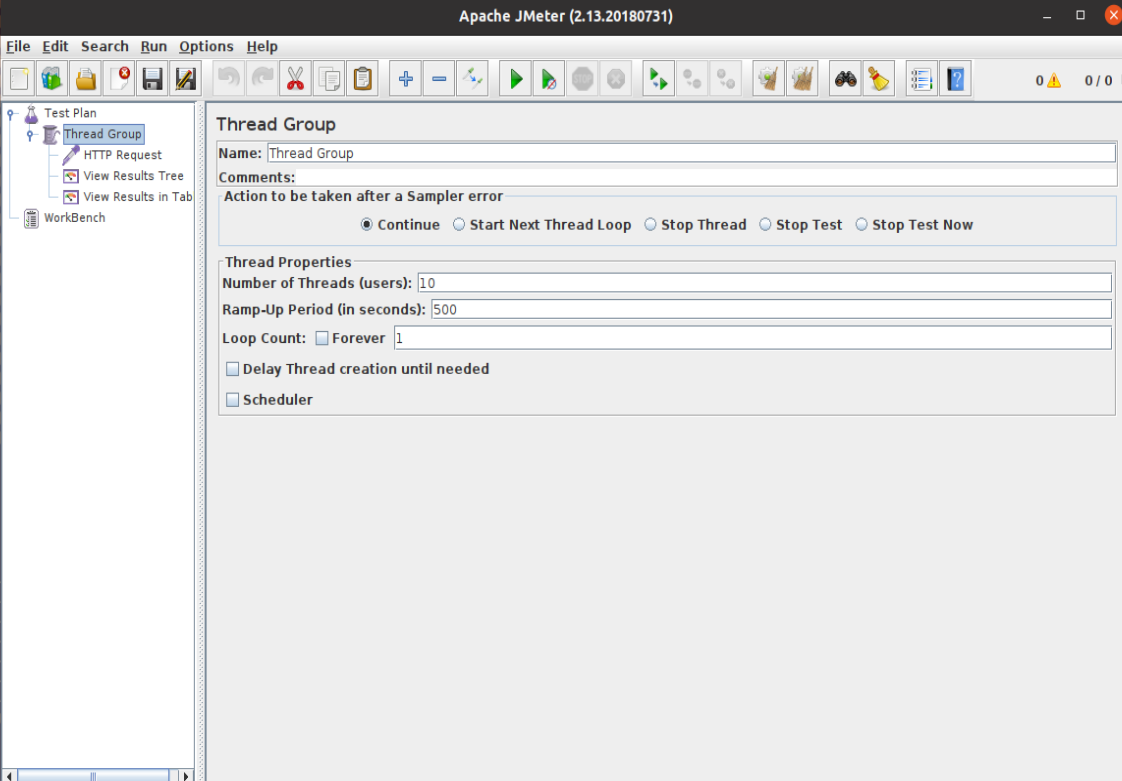
\includegraphics[scale=0.6]{tp_sosd_c1}
	\end{figure}

	\newpage
	
	\begin{figure}[!htb]
		\centering
		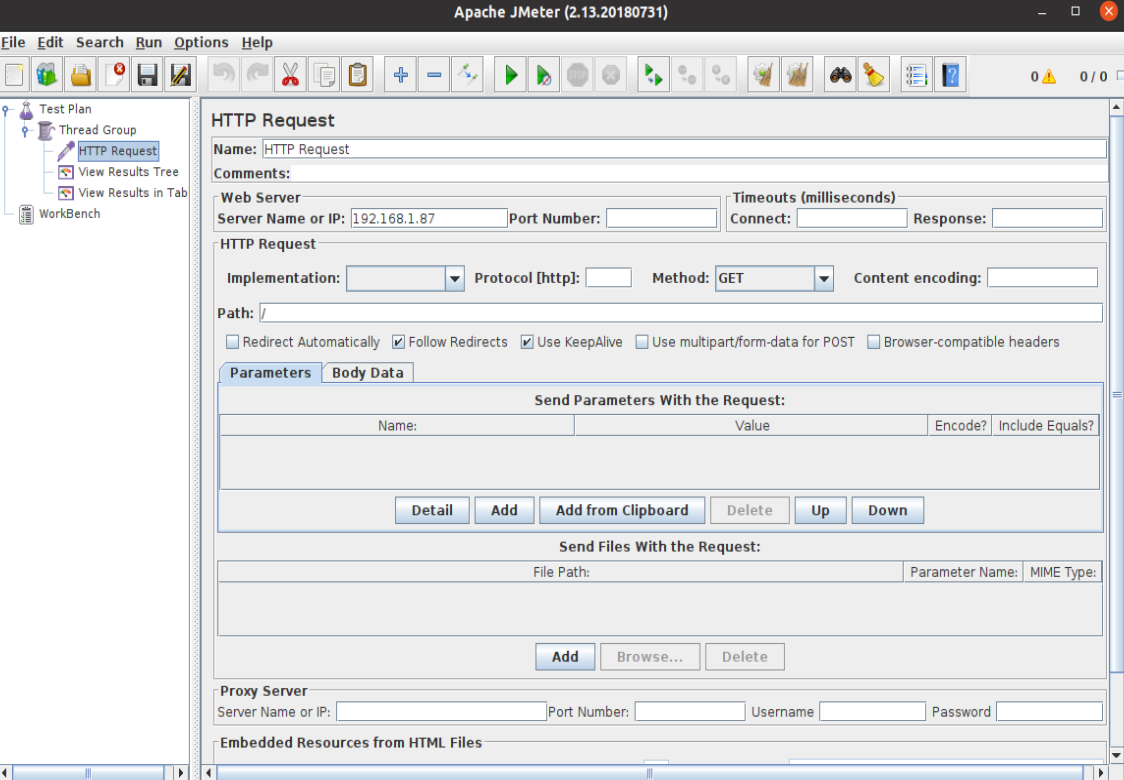
\includegraphics[scale=0.6]{tp_sosd_c2}
	\end{figure}
	\newpage
	
	\begin{figure}[!htb]
	\centering
	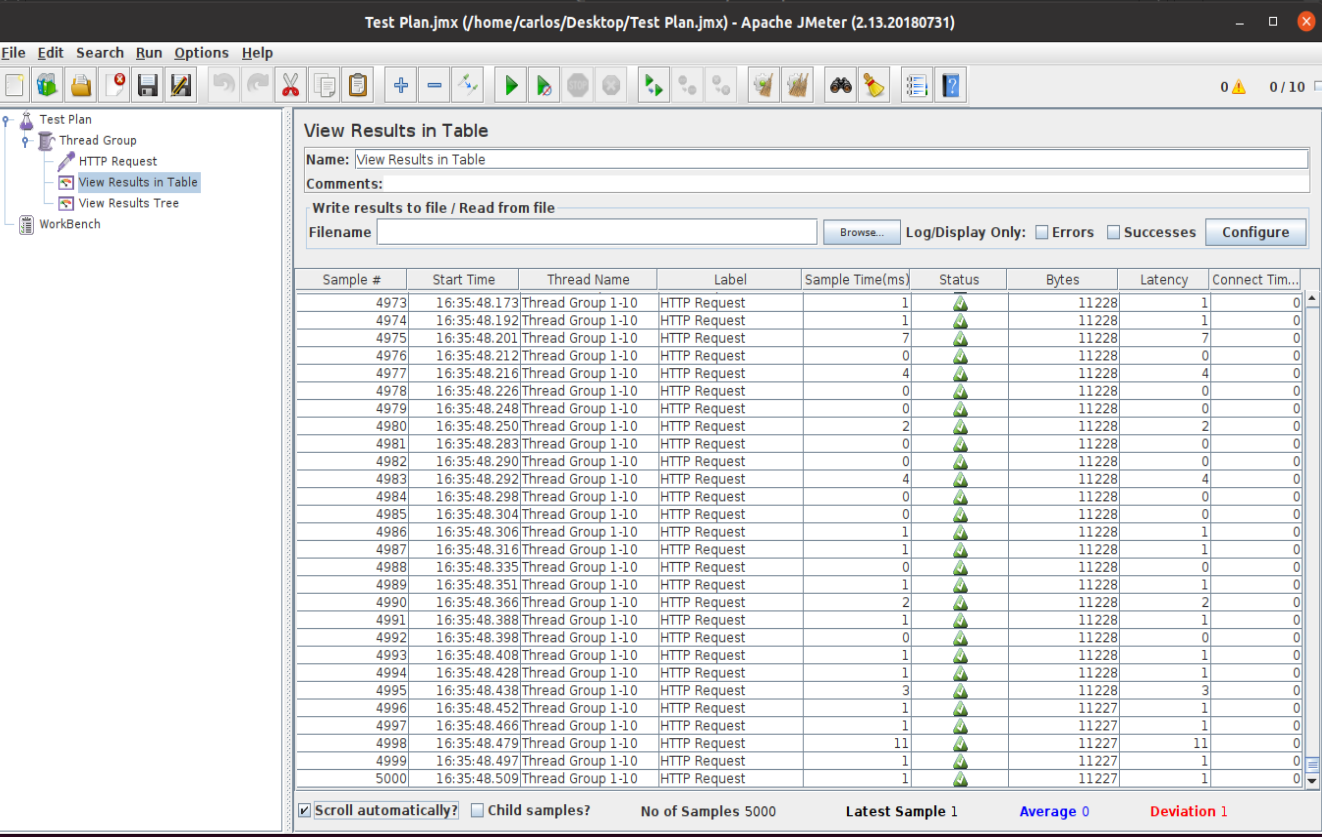
\includegraphics[scale=0.5]{tp_sosd_c3}
	\end{figure}

	\newpage
	
	\begin{figure}[!htb]
		\centering
		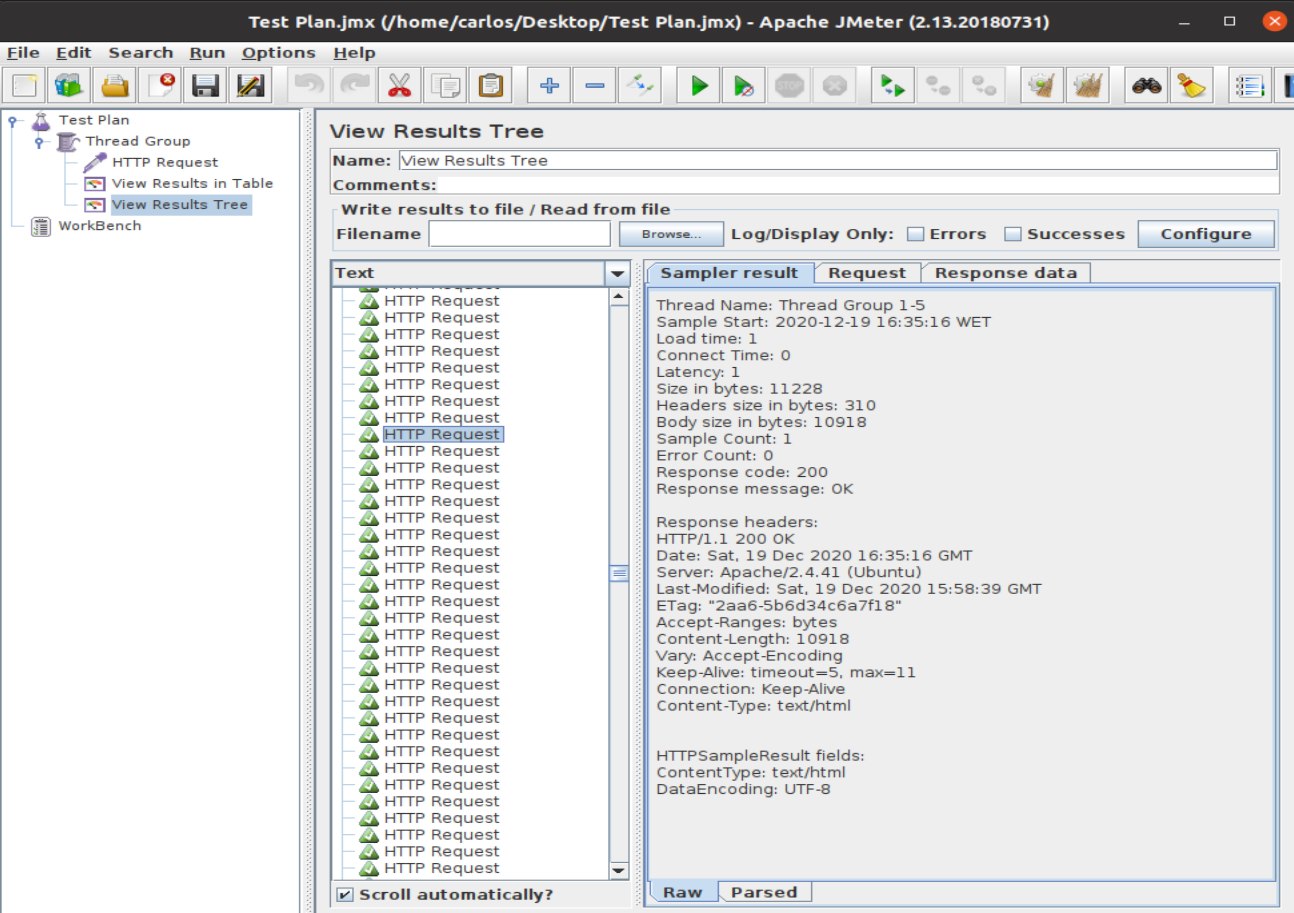
\includegraphics[scale=0.5]{tp_sosd_c4}
	\end{figure}

	\newpage
	d) Tendo como base o problema de copiar um ficheiro da primeira máquina
	virtual para a segunda máquina virtual (este ficheiro deverá ser criado na
	directoria /home/<nomeutilizador>/, com o nome sosd.txt e com o conteúdo
	“este ficheiro é para copiar”), indique os comandos que permitem realizar esta
	operação.
	Faça uso das seguintes sugestões de comandos para apresentar até 3 possíveis
	soluções distintas:
	1) scp
	2) dd, nc, pipe (|)
	3) cat, ssh, pipe (|)
	Apresente o comando para cada uma das três possíveis soluções com uma
	descrição de cada uma delas, indicando qual a melhor em termos de utilização
	de recursos e rapidez.
	vspace{2 em}
	
	\begin{figure}[!htb]
		\centering
		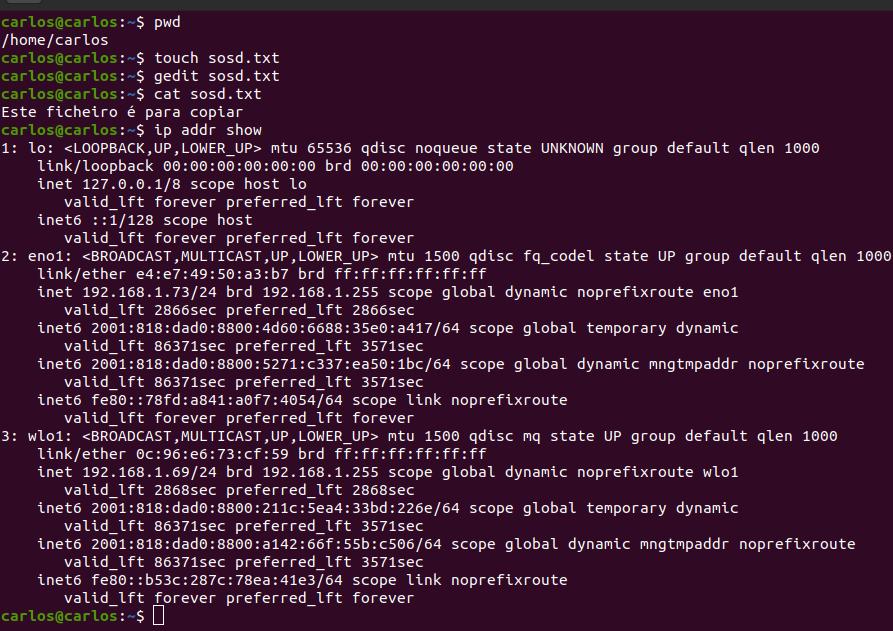
\includegraphics[scale=0.5]{tp_sosd_d1}
	\end{figure}
	
	\vspace{2 em}
	
	\begin{figure}[!htb]
		\centering
		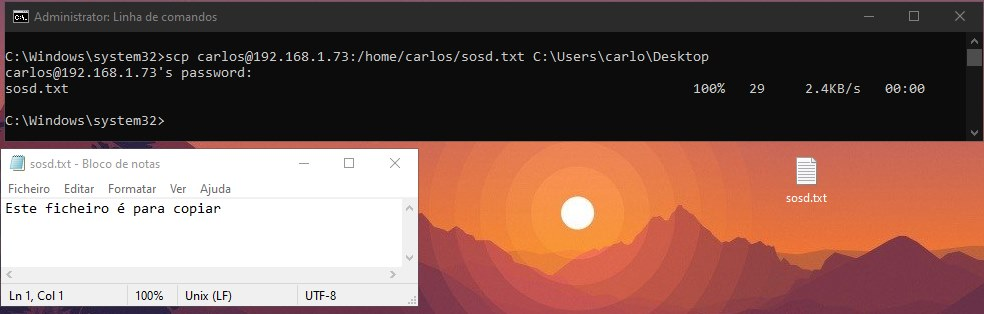
\includegraphics[scale=0.5]{tp_sosd_d2}
	\end{figure}

	%% Pagina 7
	\newpage
	\centerline{\textbf{Conclusão}}
	\vspace{5 em}
	
	Na nossa opinião foi muito interessante o desenvolvimento deste projeto, pois potenciou a experiência do desenvolvimento de Software. Assimilar os conteúdos da Unidade Curricular, desenvolver Capacidades de programação em \textit{C}\\
	
	\vspace{1 em}
	Sentimos que este projeto foi bastante exigente e fez com que nos dedicássemos mais e consequentemente melhorar as nossas capacidades.
	\\
	
	\vspace{1 em}
	Com este Trabalhos adquirimos inúmeras valias que nos serão úteis em futuros projetos.
	\\
	
	\vspace{1 em}
	Em suma, abordamos todos os assuntos lecionados e graças a isso conseguimos cumprir os objetivos propostos.
	\\
	
	% ------ Pagina 8
	\newpage

	\centerline{\textbf{Execução das Tarefas}}
	
	\vspace{3 em}
	\begin{enumerate}
		\item Parte 1 \\
			a) João Ricardo Nº 18845 \\
			b) João Ricardo Nº 18845 \\ 
			c) Carlos Santos Nº 19432 \\
			d) João Rodrigues Nº 19431 \\
			e) João Ricardo Nº 18845  \\
			f) João Rodrigues Nº 19431 \\
		\item Parte 2 \\ Carlos Santos Nº 19432 \\ João Ricardo Nº 18845 
		\item Parte 3 \\ Carlos Santos Nº 19432
	\end{enumerate}
	\vspace{3 em}
	
\end{document}